\documentclass[12pt]{article}
\usepackage{amsmath,amsfonts}
\usepackage{enumerate}
\usepackage{graphicx}
\usepackage{float}
\usepackage{multirow}
\usepackage{booktabs}

\renewcommand{\baselinestretch}{1}
\topmargin 0in \headheight 0.0in \textheight 9in \textwidth 6.5in
\oddsidemargin 0.1in \evensidemargin 0.1in

\graphicspath{{/Users/siyangren/Documents/ra-cida/ESFGSP_Paper/Simulations/results/figures}}


\begin{document}

\section*{Methods}

In this study, we conducted two simulations to evaluate the performace of LASSO
models in identifying important features in high-dimensional data. The first
simulation assumes sparsity of the features in the pixel space, while the
second simulation assumes sparsity in the frequency space.

The pixel space refers to the original high-dimensional space where each
dimension represents a pixel in an image. In this space, features are directly
observed and may have inherent correlations. Conversely, the frequency space is
a transformed version of the pixel space, obtained through techniques like
eigen decomposition.

Suppose \( X \) is a column vector representing 256 pixels. Its covariance
matrix, \( \Sigma \), is defined to have an exponential correlation structure,
where \( \Sigma_{i j}=-\exp (\operatorname{dist}(i, j)) \). Here, \(
\operatorname{dist}(i, j) \) is the distance between the pixels \( i \) and \(
j \) in a \( 16 \times 16 \) matrix.

Let \( V \) be the matrix of eigenvectors of \( \Sigma \), with each column
representing an eigenvector. We can transform the random vector \( X \) into
the frequency space by \( X_{\text {freq }}=V^T X \). The covariance matrix of
\( X_{\text {freq }} \) is given by \(
\operatorname{cov}\left(X_{\mathrm{freq}}\right)=V^T \Sigma V \), which is a
diagonal matrix.

For the simulations, in each iteration, we randomly generate \( X_{\text {freq
}} \) from a multivariate normal distribution with the covariance matrix
\(\operatorname{cov}\left(X_{\text {freq }}\right) \). We repeat this process
1000 times. Then, we calculate \( X \) as \( X=V X_{\text {freq }} \).

In the first simulation, we assume sparsity in the coefficient vectors in the
pixel space. The coefficient vector \( \beta \) was specified to have non-zero
values exclusively within a central \( 8 \times 8 \) region. The response
variable \( y \) was drawn from a binomial distribution with success
probabilities determined by \( \eta = X \beta \). The non-zero coefficients in
\( \beta \) were chosen such that the probability \( p = \frac{1}{1 +
\exp(-\eta)} \) was uniformly distributed across interval \( [0, 1] \).

In the second simulation, we assume sparsity in the coefficient vectors in the
frequency space. We defined a sparse coefficient vector \( b \) in the
frequency space, where most of the 256 entries were zero and a randomly 10\%
were non-zero. The response variable \( y \) was generated similarly to the
first simulation, ensuring \( p = \frac{1}{1 + \exp(-\eta)} \) was evenly
distributed.

For both simulations, we fit two models: one using the covariates in the pixel
space and another using the covariates in the frequency space. Each dataset,
generated in size \( 1000 \times 256 \) and representing images of \( 16 \times
16 \) pixels, was split into training (80\%) and test (20\%) sets. The
regularization parameter \( \lambda \) was tuned using cross-validation with
the default binomial deviance metric. The dataset was divided into 10 folds,
with the model trained and validated iteratively across these folds, varying \(
\lambda \). Here we use two \( \lambda \) values, `lambda.min` is the
regularization value that minimizes cross-validated error, and `lambda.1se` is
the largest lambda within one standard error of the minimum.

After selecting the optimal \( \lambda \), model performance was evaluated
using accuracy and AUC metrics. Additionally, a permutation test was conducted
100 times to calculate p-values for each covariate. Across all iterations, we
calculated the mean and standard deviation of the metrics, as well as the
percentage of significant p-values for each covariate.


\section*{Results}


\begin{figure}[H] 
	\centering
	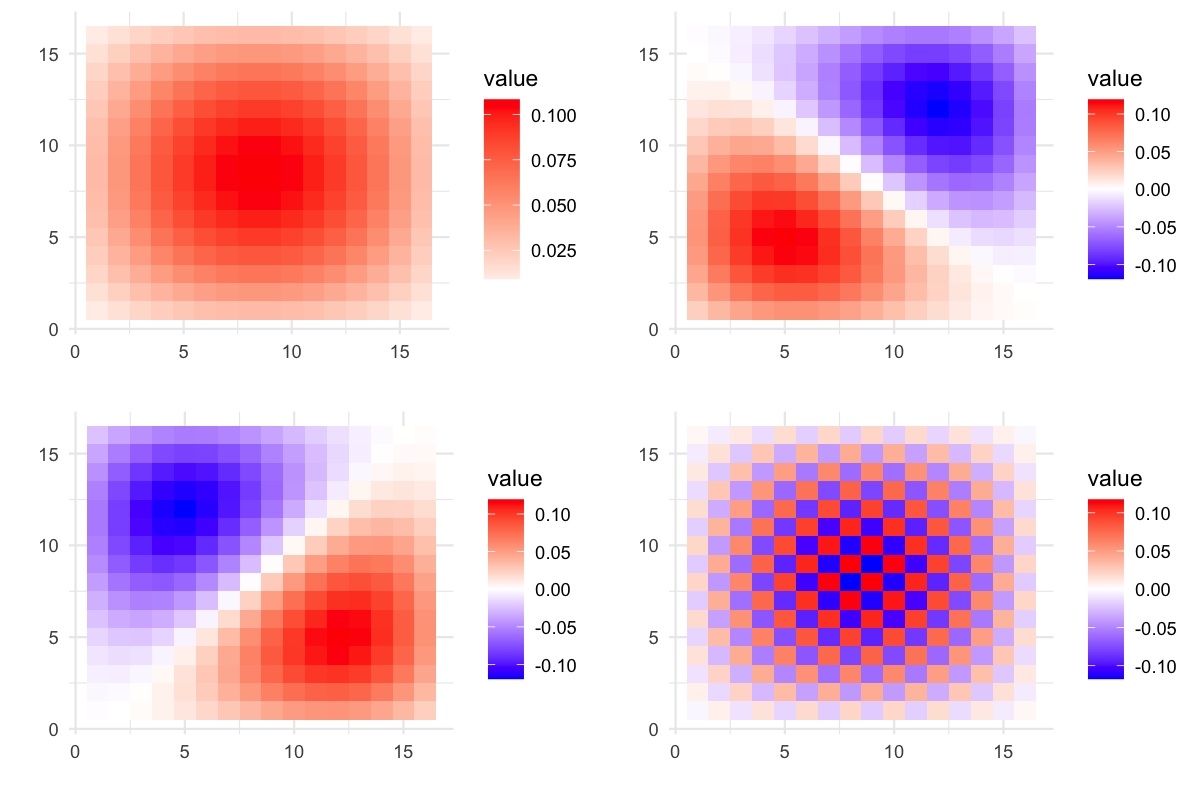
\includegraphics[width=\textwidth]{top_bottom_eigvecs.png} 
\caption{Frequencies associated with the top three eigenvalues (top row and
bottom left) and the frequency associated with the smallest eigenvalue (bottom
right), highlighting the primary and least significant patterns in the pixel
space.}
	\label{fig:top_bottom_eigvecs} 
\end{figure}

Figure~\ref*{fig:top_bottom_eigvecs} shows the frequencies tied to the top
three eigenvalues representing the main patterns in the pixel space. The
frequency associated with the smallest eigenvalue highlights the least
significant variance.

\begin{figure}[H] 
	\centering
	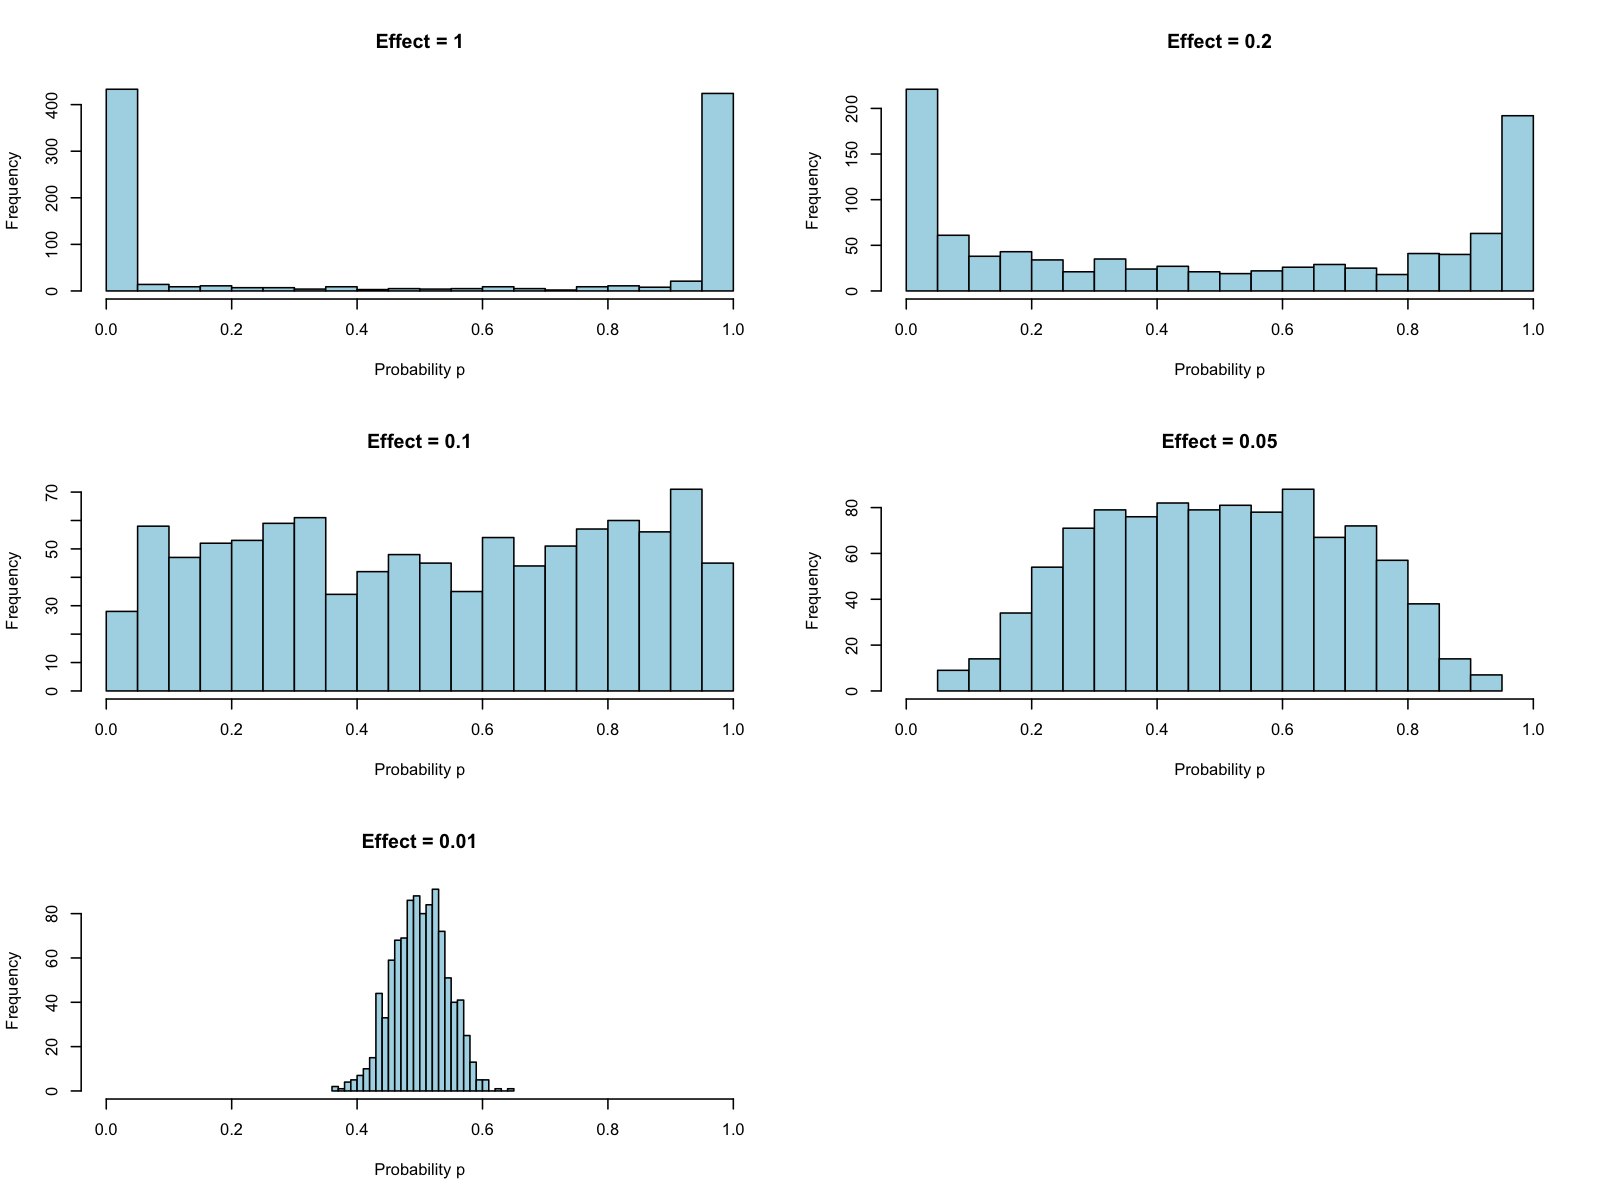
\includegraphics[width=\textwidth]{sim1_p_dist.png} 
	\caption{The distribution of \(p\) at different \(\beta\) values. \(\beta = 0.1\) was
chosen for model fitting as it gives the most evenly distributed values.}
	\label{fig:sim1_p_dist} 
\end{figure}

In Simulation 1, the distribution of the success probability \( p \) was
evaluated at various \( \beta \) values: 0.01, 0.05, 0.1, 0.2, and 1. Figure
\ref{fig:sim1_p_dist} shows that \( \beta = 0.1 \) resulted in the most even
spread of \( p \), making it the optimal choice for model fitting.

\begin{figure}[H] 
	\centering
	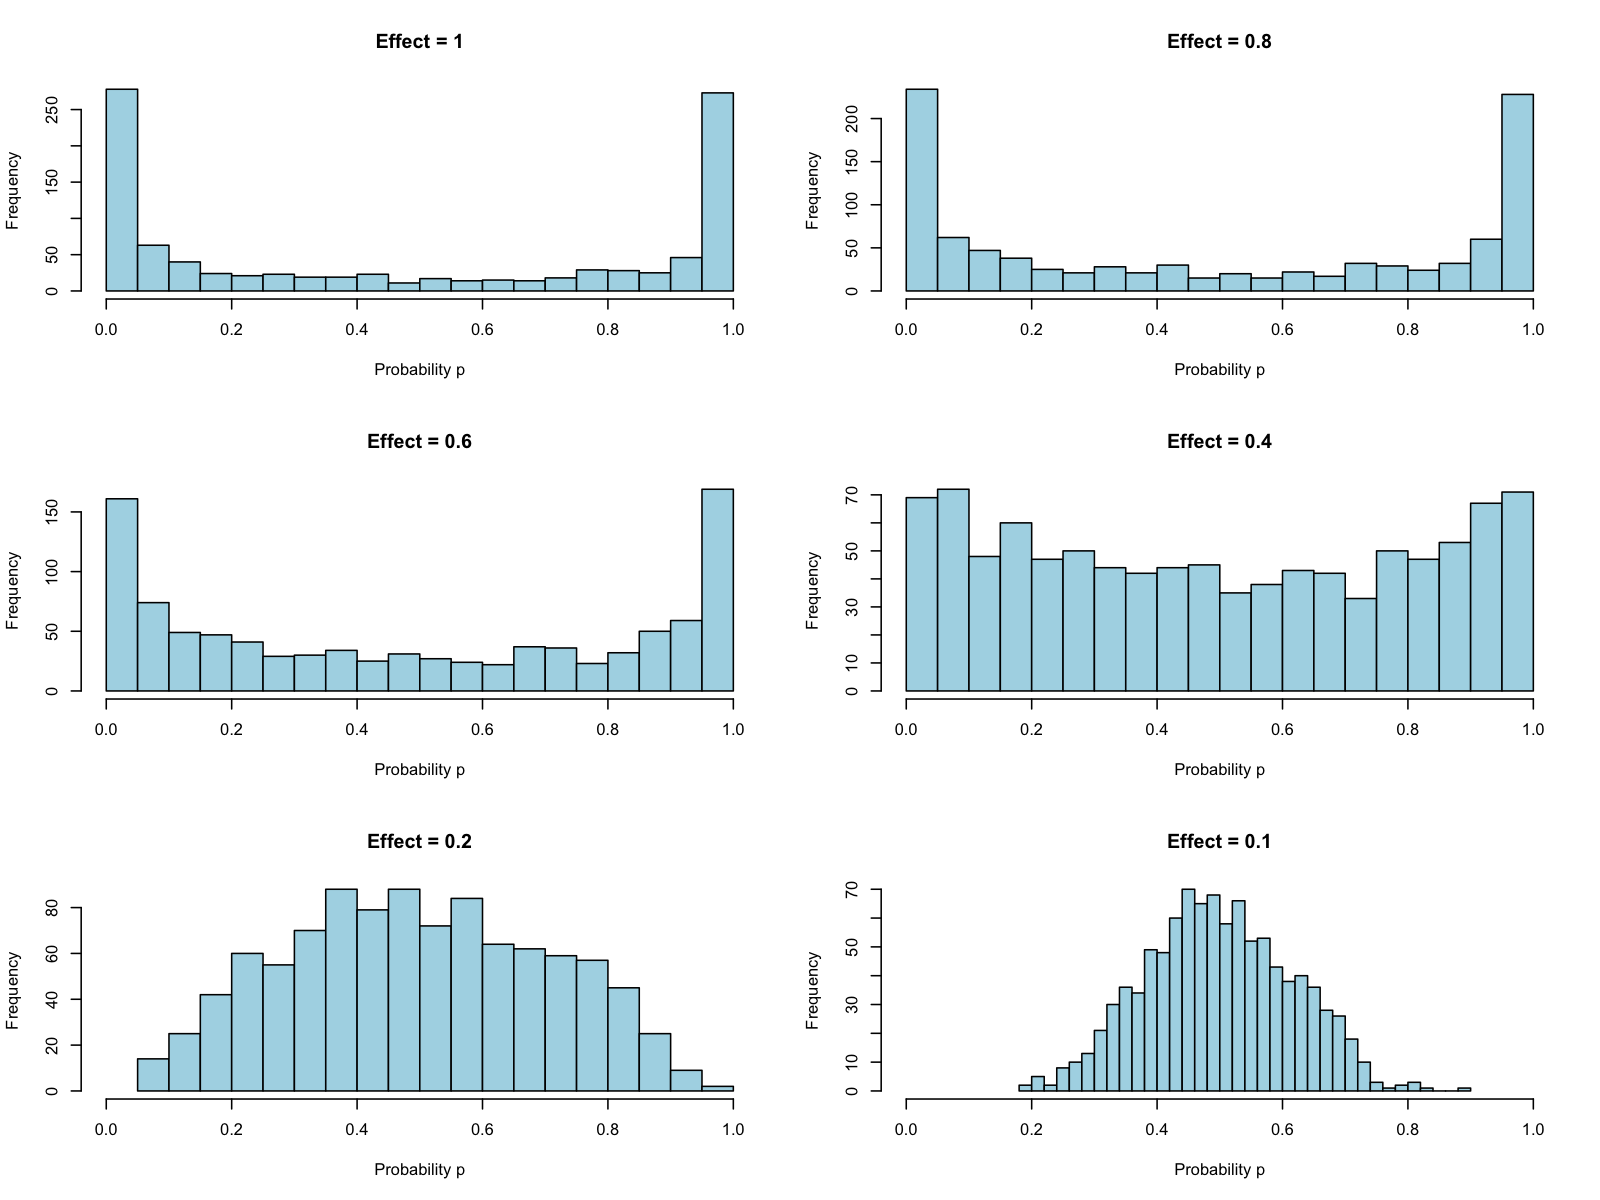
\includegraphics[width=\textwidth]{sim2_p_dist.png} 
	\caption{The distribution of \(p\) at different \( b \) values. \( b = 0.4 \) was
chosen for model fitting as it gives the most evenly distributed values.}
	\label{fig:sim2_p_dist} 
\end{figure}

In Simulation 2, the effect size \( b \) was varied at 0.1, 0.2, 0.4, 0.6,
0.8, and 1. Figure \ref{fig:sim2_p_dist} shows that \( b = 0.4 \) yielded the most
evenly distributed \( p \), indicating it as the best choice for the model.

\begin{figure}[h!]
	\centering
	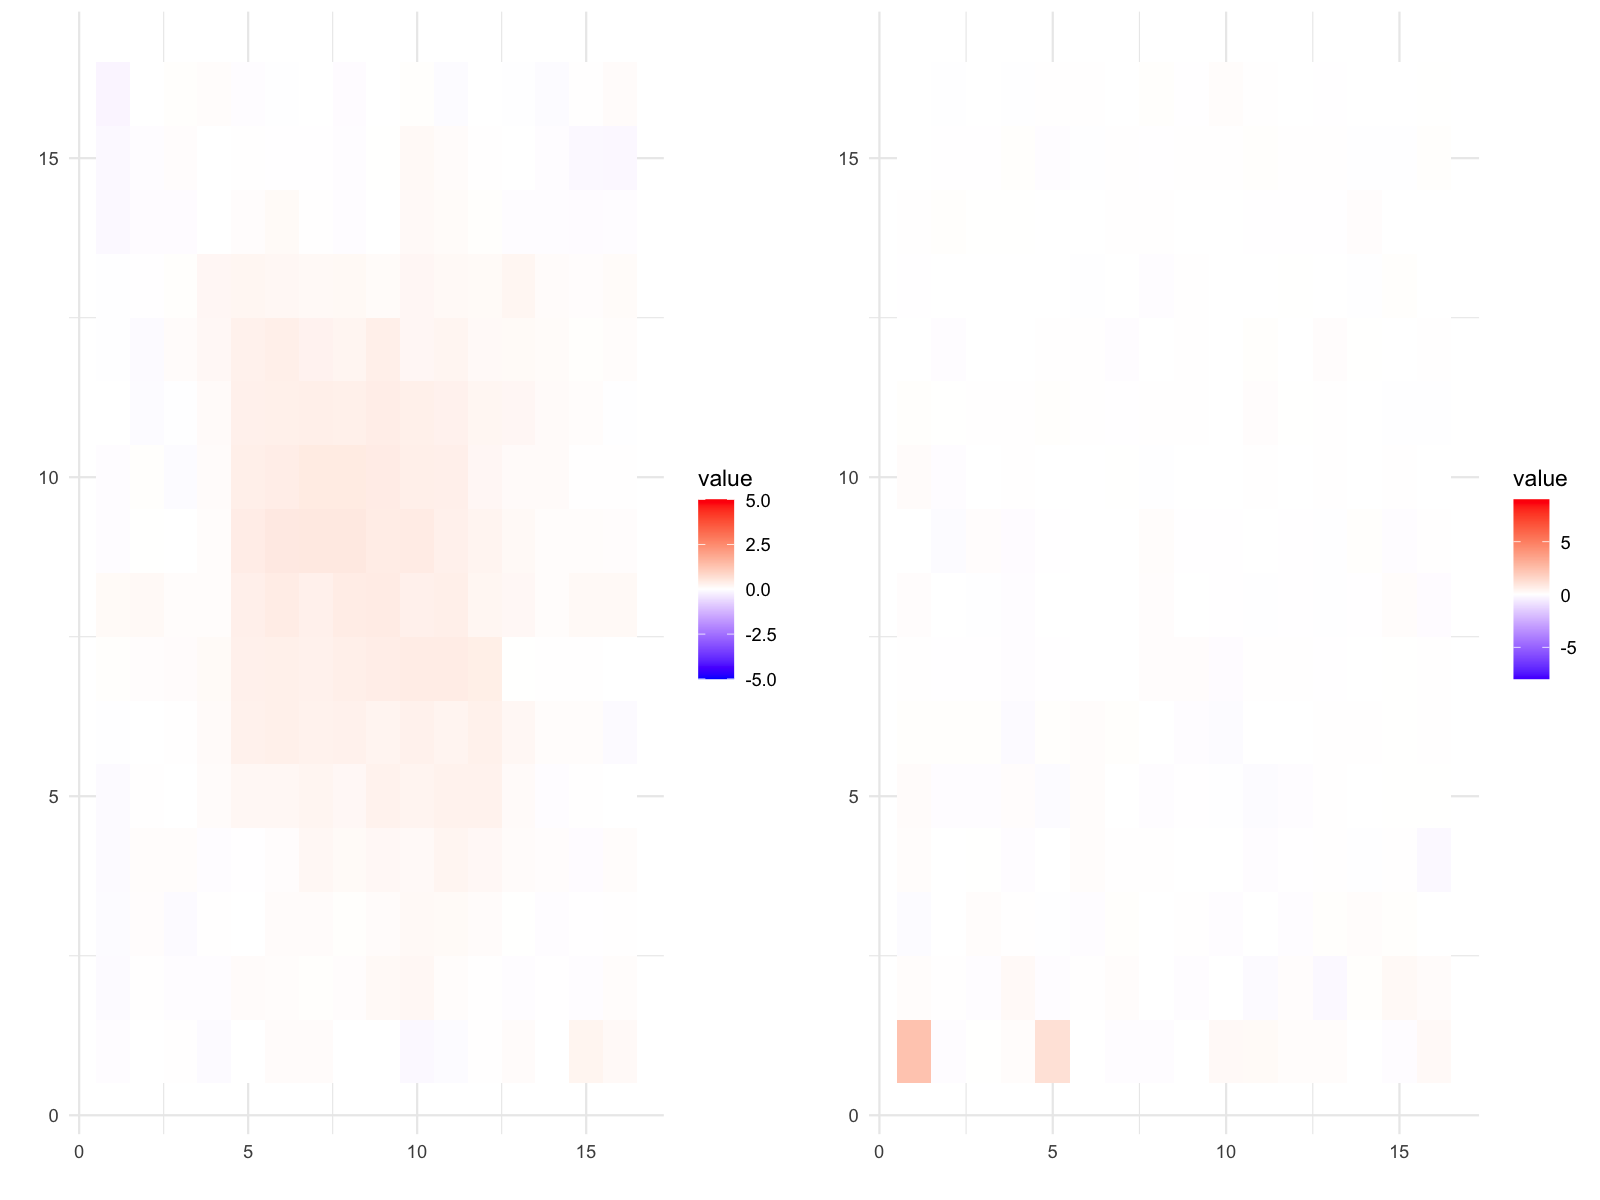
\includegraphics[width=0.8\textwidth]{group_diff_sim1.png}
	\caption{The group mean difference between \( y = 1 \) and \( y = 0 \) in
	the pixel space and frequency space.}
	\label{fig:group_diff1}
\end{figure}

\begin{figure}[h!]
	\centering
	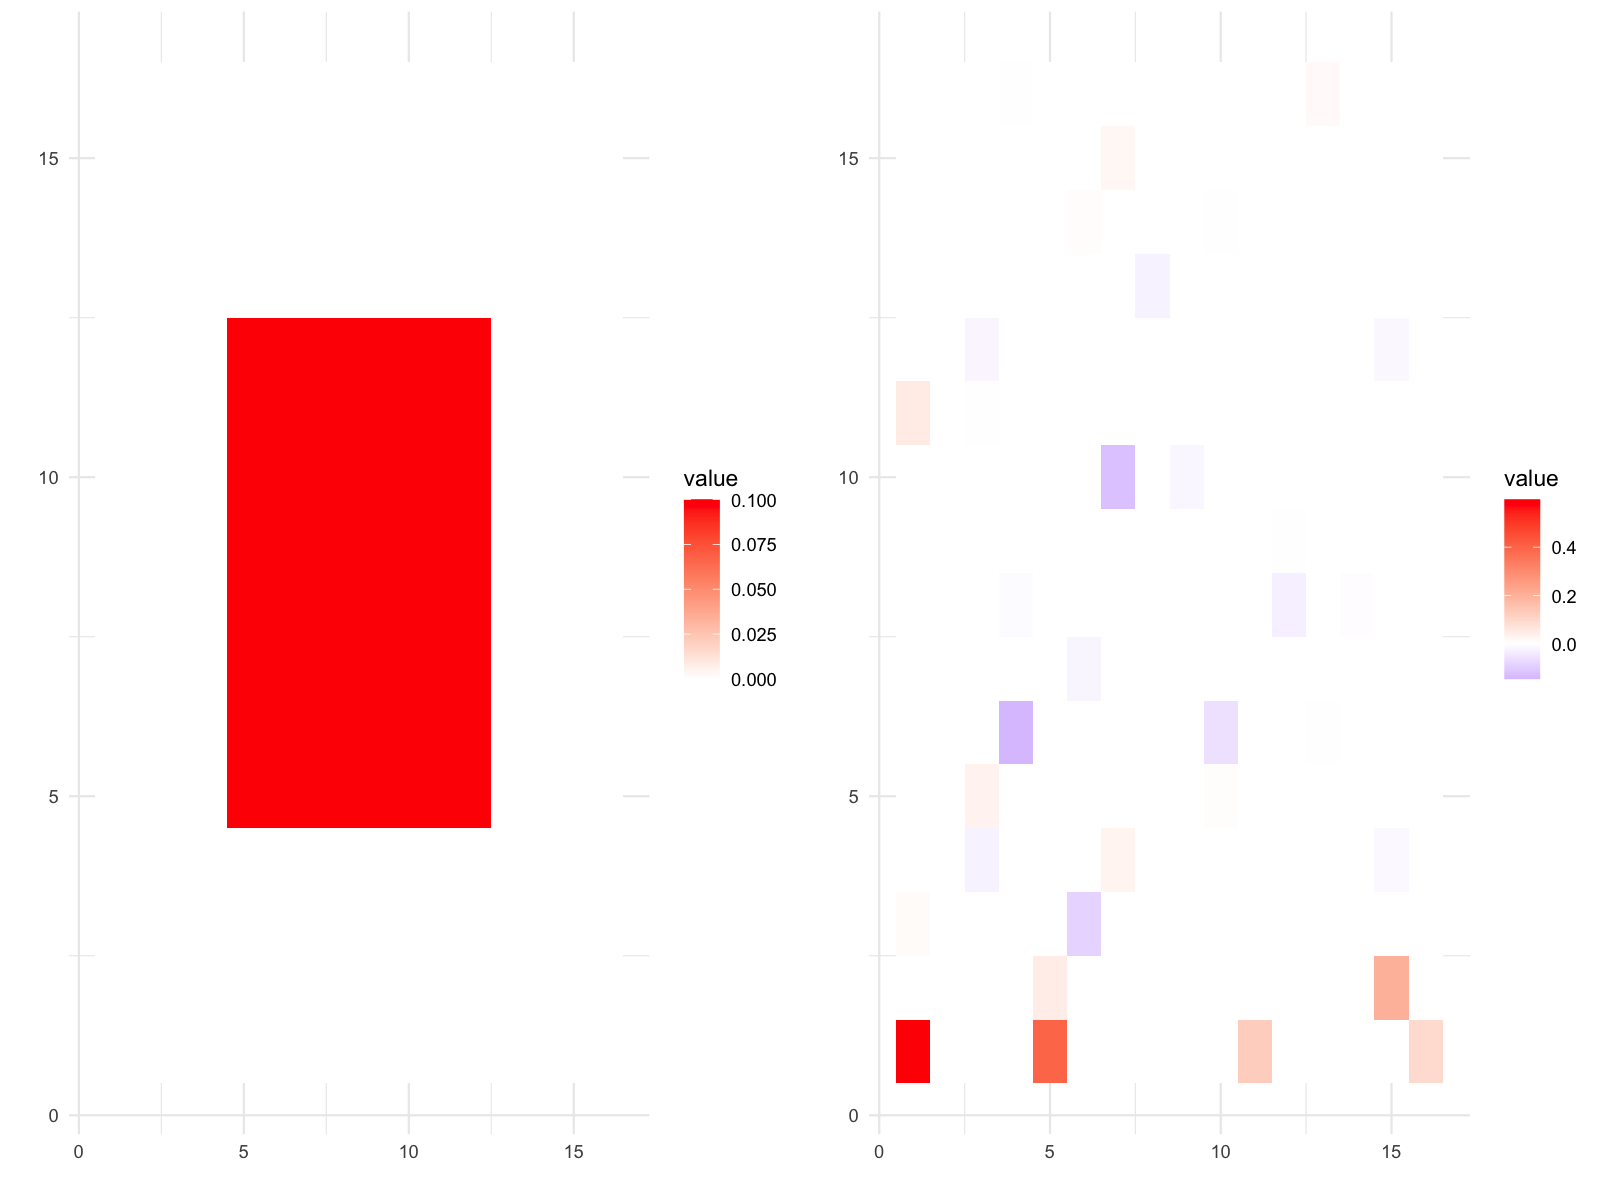
\includegraphics[width=0.8\textwidth]{coefs_sim1.png}
  \caption{Coefficients for Simulation 1 in the pixel space (left) and
	frequency space (right).}
  \label{fig:coefs_sim1}
\end{figure}

Figure \ref{fig:group_diff1} shows the group mean difference in the covariate
values between instances where \( y=1 \) and \( y=0	\) in both the pixel space
and the frequency space. The heatmaps illustrate that in the pixel space, the
central region with non-zero coefficients in \( \beta \) corresponds to higher
mean values of the covariates. Indicating its strong association with the
positive response. In the frequency space, the pattern is more dispersed but
still reflects the influence of the non-zero coefficients.

Figure \ref{fig:coefs_sim1} presents the coefficients for Simulation 1, where
sparsity was assumed in the pixel space. The coefficients exhibit a
concentrated non-zero region in the center of the image, reflecting the
assumption that only a central subset of the covariates significantly
influences the response variable. This central region aligns with the higher
mean values observed in the pixel space's covariates, as shown in Figure
\ref{fig:group_diff1}.


\begin{figure}[h!]
	\centering
	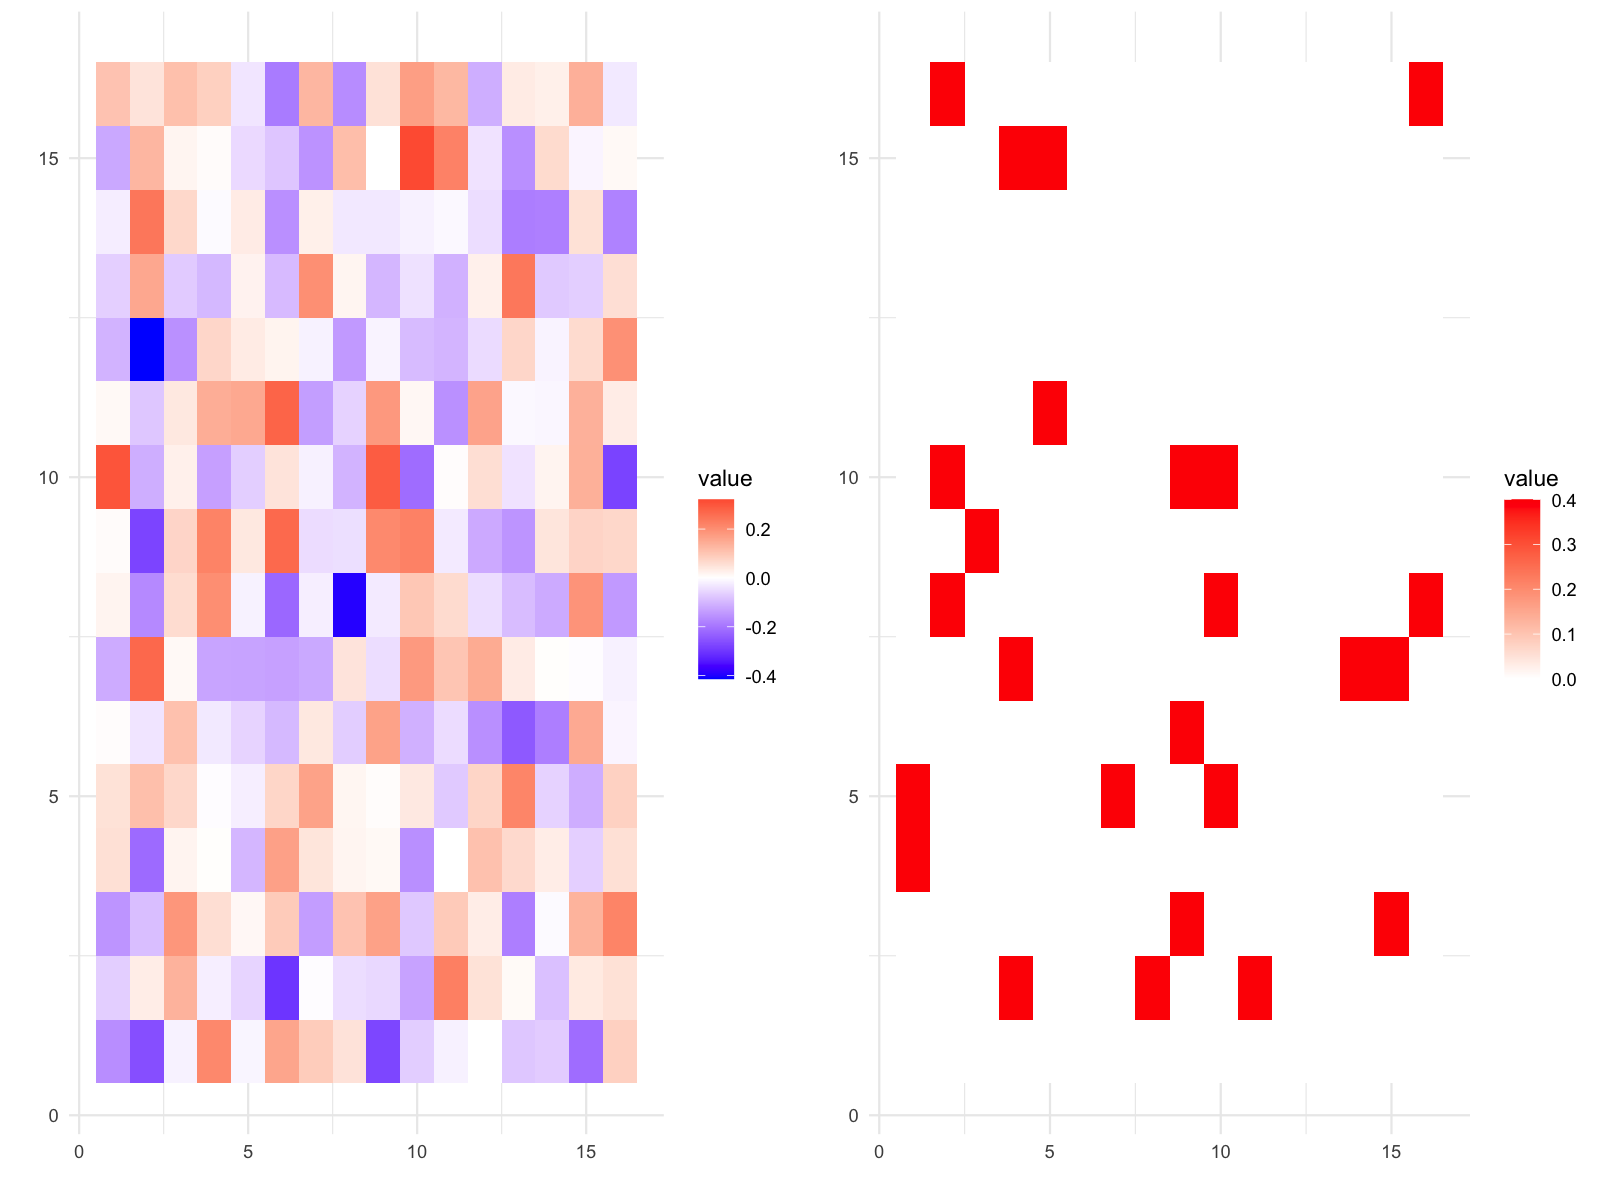
\includegraphics[width=\textwidth]{coefs_sim2.png}
  \caption{Coefficients for Simulation 2.}
  \label{fig:coefs_sim2}
\end{figure}

\begin{figure}[h!]
	\centering
	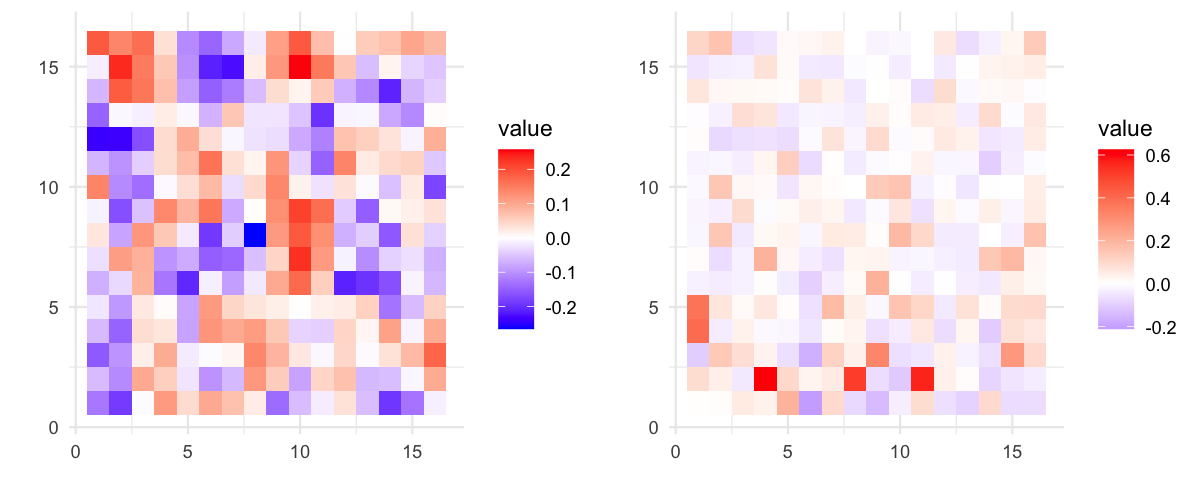
\includegraphics[width=\textwidth]{group_diff_sim2.png}
	\caption{The group mean difference between \( y = 1 \) and \( y = 0 \).}
	\label{fig:group_diff2}
\end{figure}

Table~\ref*{tab:auc_acc_table} shows the average AUCs and accuracys calculated
by fitting models on the 1000 simulated dataset, on both the frequency sapce
and pixel space. We can see that no matter we assume sparsity in coefficient
vectors in the pixel space of the frequency space, fitting models on the
frequency space provides better performance in AUCs and accuracys. When
assuming sparsity in coefficient vectors in the pixel space and using
`lambda.min` as the regularization value, models fitting with covariates in
the pixel space \( (X) \) achieves an AUC of 0.803 (se = 0.031), and an
accuracy of 72.5\% (se = 0.032); while models fitting with covariates in the
corresponding frequency space \( (X_{\text{freq}}) \) achieves a slightly
better AUC of 0.827 (se = 0.029) and better accuracy of 74.6\% (se = 0.031).
We see a similar advantage of fitting models on the frequency space when
assuming sparsity in coefficient vectors in the frequency space, and using
either `lambda.min` or `lambda.1se` does not affect this advantage.

\begin{table}[h!]
\centering
\caption{}
\label{tab:auc_acc_table}
\begin{tabular}{l|cc|cc}
\toprule
& \multicolumn{2}{c}{Model on the pixel space} & \multicolumn{2}{c}{Model on the freq space} \\ 
	Lambda & AUC (SE) & Accuracy (SE) & AUC (SE) & Accuracy (SE) \\ 
\midrule
	lambda.min & 0.803 (0.031) & 0.725 (0.032) & 0.827 (0.029) & 0.746 (0.031) \\
	lambda.1se & 0.800 (0.031) & 0.723 (0.032) & 0.826 (0.029) & 0.745 (0.031) \\ 
	lambda.min & 0.756 (0.036) & 0.687 (0.035) & 0.816 (0.032) & 0.735 (0.033)  \\
	lambda.1se & 0.734 (0.040) & 0.669 (0.036) & 0.816 (0.032) & 0.734 (0.034) \\
\bottomrule
\end{tabular}
\end{table}

Then, for both Simulation 1 and Simulation 2, we fitted two models, one using
covariates on the frequency space, another using covariates on the pixel
space. In 

\end{document}
